\section{Least and Greatest Element}
\label{tree:poset:leastandgreatest}

An other term that we might want to add to our vocabulary is a term that refers
to the element $x \in \P$ for which $y \geq x, \forall y \in \P$. In this case,
we say that $x$ is the least element, note that not every poset has such an
element. The least element is written $\hat{0}$ and if there is a $\hat{0}$ in
$\P$ we say that $\P$ has a $\hat{0}$. Similarly we define the greatest element
$\hat{1}$ such that $x \leq \hat{1}$ for all $x \in \P$.

\begin{figure}
	\centering
	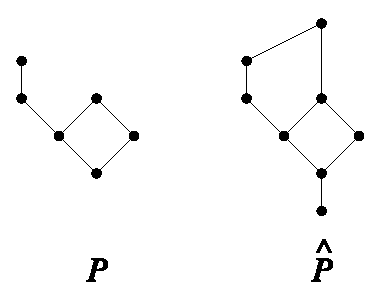
\includegraphics[height=0.2\textheight]{fig/stanley/3-3}
	\caption{\label{fig:stanley:3-3} Adjoining a $\hat{0}$ and $\hat{1}$, from
\citet*{Stanley:2011:ECV:2124415}.}
\end{figure}

We define the operation of adjoining a $\hat{0}$ and $\hat{1}$ to a poset $\P$,
even if $\P$ already has a $\hat{0}$ or a $\hat{1}$. The resulting poset of this
operation is denoted $\hat{\P}$. In \ref{fig:stanley:3-3} we see an example of
this operation applied to some poset.



